
\documentclass[
12pt,
a4paper,
pdftex,
czech,
titlepage
]{report}

\usepackage{float}
\usepackage[czech]{babel}
\usepackage[utf8]{inputenc}
\usepackage{lmodern}
\usepackage{textcomp}
\usepackage[T1]{fontenc}
\usepackage{amsfonts}
\usepackage{titlesec}
\usepackage{graphicx}
\usepackage{longtable}
\usepackage{multirow}
\usepackage{tabularx} 
\usepackage[unicode]{hyperref}
\usepackage{indentfirst}
\usepackage{listings}
\usepackage{xcolor}
\hypersetup{
    colorlinks=true,
    citecolor=green,
    filecolor=black,
    linkcolor=black,
    urlcolor=magenta
}
\lstset{%
    backgroundcolor=\color{yellow!20},%
    basicstyle=\small\ttfamily\color{blue},%
    }%
\lstset{emph={%  
    IDENT, ASSIGN, SEMI, ident%
    },emphstyle={\color{brown}}%
}%

\titleformat{\chapter}
  {\normalfont\LARGE\bfseries}{\thechapter}{1em}{}
\titlespacing*{\chapter}{0pt}{0ex plus 1ex minus .2ex}{2.0ex plus .2ex}
\titleclass{\subsubsubsection}{straight}[\subsection]


\begin{document}

\begin{titlepage}
	\vspace*{-2cm}
	{\centering
\includegraphics[scale=1.5]{FAV_logo.pdf}\par}
	\centering
	\vspace*{2cm}
	{\Large Dokumentace k semestrální práci z KIV/FJP\par}
	\vspace{1.0cm}
	{\Huge\bfseries Překladač jazyka Pascal0Like\par}
	\vspace{7cm}

	\begin{flushleft} 
	\begin{table}[ht]
	\label{stats}
	\begin{tabular}{ll}
	\textbf{Student:}  & Martin Kružej, Jakub Šmaus   \\
	\textbf{St. číslo:}   & A17N0079P, A17N0089P    \\
	\textbf{E-mail:}  & kruzej@students.zcu.cz, smaus@students.zcu.cz  \\
	\textbf{Datum:}    & \today            \\ 
	\end{tabular}
	\end{table}
	\end{flushleft}
	
	\vfill


\end{titlepage}

\tableofcontents
\thispagestyle{empty}
\clearpage

\chapter{Zadání}
\setcounter{page}{1}

\section{Tvorba překladače zvoleného jazyka}
Cílem práce bude vytvoření překladače zvoleného jazyka. Je možné inspirovat se jazykem PL/0, vybrat si podmnožinu nějakého existujícího jazyka nebo si navrhnout jazyk zcela vlastní. Dále je také potřeba zvolit si pro jakou architekturu bude jazyk překládán (doporučeny jsou instrukce PL/0, ale je možné zvolit jakoukoliv instrukční sadu pro kterou budete mít interpret). 

Jazyk musí mít minimálně následující konstrukce:

\begin{itemize}
\item definice celočíselných proměnných
\item definice celočíselných konstant
\item přiřazení
\item základní aritmetiku a logiku (+, -, *, /, AND, OR, negace a závorky, operátory pro porovnání čísel)
\item cyklus (libovolný)
\item jednoduchou podmínku (if bez else)
\item definice podprogramu (procedura, funkce, metoda) a jeho volání
\end{itemize}

Překladač který bude umět tyto základní věci bude hodnocen deseti body. Další body (alespoň do minimálních 20) je možné získat na základě rozšíření, jsou rozděleny do dvou skupin, jednodušší za jeden bod a složitější za dva až tři body. Další rozšíření je možno doplnit po konzultaci, s ohodnocením podle odhadnuté náročnosti.\newline
\textbf{Jednoduchá rozšíření (1 bod):}
\begin{itemize}
\item každý další typ cyklu (for, do .. while, while .. do, repeat .. until, foreach pro pole)
\item else větev
\item datový typ boolean a logické operace s ním
\item datový typ real (s celočíselnými instrukcemi)
\item datový typ string (s operátory pro spojování řětezců)
\item rozvětvená podmínka (switch, case)
\item násobné přiřazení (a = b = c = d = 3;)
\item podmíněné přiřazení / ternární operátor (min = (a < b) ? a : b;)
\item paralelní přiřazení ({a, b, c, d} = {1, 2, 3, 4};)
\item příkazy pro vstup a výstup (read, write -- potřebuje vhodné instrukce které bude možné využít)
\end{itemize}
\textbf{Složitější rozšíření (2 body):}
\begin{itemize}
\item příkaz GOTO (pozor na vzdálené skoky)
\item datový typ ratio (s celočíselnými instrukcemi)
\item složený datový typ (Record)
\item pole a práce s jeho prvky
\item operátor pro porovnání řetězců
\item parametry předávané hodnotou
\item návratová hodnota podprogramu
\item objekty bez polymorfismu
\item anonymní vnitřní funkce (lambda výrazy)
\end{itemize}
\textbf{Rozšíření vyžadující složitější instrukční sadu než má PL/0 (3 body):}

\begin{itemize}
\item dynamicky přiřazovaná paměť -- práce s ukazateli
\item parametry předávané odkazem
\item objektové konstrukce s polymorfním chováním
\item instanceof operátor
\item anonymní vnitřní funkce (lambda výrazy) které lze předat jako parametr
\item mechanismus zpracování výjimek
\end{itemize}

Vlastní interpret (řádkový, bez rozhraní, složitý alespoň jako rozšířená PL/0) je za 6 bodů. 

\section{Bodované náležitosti}

Kromě toho že by program měl fungovat se zohledňují i další věci, které mohou pozitivně nebo negativně ovlivnit bodování:

\begin{itemize}
\item testování -- tvorba rozumné automatické testovací sady +3 body (pro inspiraci hledejte test suit pro LLVM nebo se podívejte na \href{http://www.plumhall.com/suites.html}{Plum Hall testy}, ale jde skutečně jen o inspiraci, stačí výrazně jednodušší řešení). Užitečné a stručné povídání na dané téma najdete také \href{http://www.engr.mun.ca/~theo/Publications/compiler-testing.pdf}{tady}.
\item Kvalita dokumentace -x bodů až +2 body podle kvality a prohřešků (vynechaná gramatika, nesrozumitelné věty, příliš chyb a překlepů, bitmapové obrázky pro diagramy s kompresními artefakty, ...).
\item Vedení projektu v GITu -x bodů až +2 body podle důslednosti a struktury příspěvků.
\item Kvalita zdrojového textu -x bodů až +2 body podle obecně známých pravidel ze ZSWI, PPA a podobně (magická čísla, struktura programu a dekompozice problému, božské třídy a metody, ...)
\end{itemize}

\chapter{Analýza}

Překladač je obecně program, který převádí zdrojový kód do nějakého cílového kódu. Zadání nespecifikuje, které tyto kódy použít a dává nám volnost použít i vlastní. Cílový kód je interpretován tzv. interpretem. Součástí zadání je i jeho implementace ohodnocená body, proto bude v této práci také vytvořen.

\section{Analýza překladače}

Základem překladače je tedy určit, jaký zdrojový kód bude překládán. Definicí tohoto kódu je gramatika. Jde o souhrn pravidel nejčastěji ve formátu \textbf{EBNF}(\textit{Extended Backus–Naur form}), která jednoznačně určují, jestli zadaný kód (či jazyk) patří či nepatří do našeho překládaného kódu. 

Další částí překladače je lexikální analyzátor. Ten projde zdrojový kód a nahradí jeho jednotlivé části tzv. tokény. Výstup tohoto analyzátoru je předán syntaktickému analyzátoru, jenž kontroluje za pomocí definované gramatiky strukturu programu. Výstupem je často derivační strom. V této chvíli je možné zdrojový program dále zpracovat, např. kontrola typů, proměnných apod. dle definovaných pravidel vlastního programovacího jazyka. Poslední částí překladače je samotný překlad do instrukcí cílové platformy. Nyní přichází na řadu program, jenž cílový kód bude interpretovat.

Pro všechny tyto komponenty bude nutné vytvořit vlastní řešení s výjimkou lexikálního/syntaktického analyzátoru, kde je možnost použít některé existující nástroje jako \textbf{YACC} a \textbf{ANTLR}. Oba dva dělají ve své podstatě to samé, jen YACC vyžaduje implementaci překladače v programovacím jazyce C, zatímco ANTLR v Javě. Jde tedy o osobní preferenci, který z těchto nástrojů použít.

Náš tým se rozhodl pro ANTLR a tedy pro Javu. Překládaný jazyk bude postaven na vyučovací gramatice PL/0, doplněn o některé vlastnosti jazyka Pascal. Samotný PL/0 je jazyk velice jednoduchý a pouhou jeho implementací by zadání nebylo splněno na požadovaný počet bodů. Původní návrh také počítá s tím, že překladač bude překládat do instrukcí PL/0 tak, aby mohl být interpretován libovolným interpretem PL/0. 

Zadání vyžaduje vedení práce na githubu, práci je tedy možno najít na adrese \href{https://github.com/SmausJakub/heine-fluch}{https://github.com/SmausJakub/heine-fluch}.

\section{Analýza jazyka}

Náš nový vlastní jazyk nese pracovní název \texttt{Pascal0Like}, protože vychází z PL/0 a Pascalu.

Z PL0 si vezmeme tyto vlastnosti:
\begin{itemize}
\item Program je tvořen blokem a končí tečkou
\item Blok je rozdělen na deklarační část a příkazovou část
\item Deklarovat je možné konstanty a proměnné
\item Příkazy jsou odděleny středníkem
\item Proměnné jsou typu číslo
\item Je možné deklarovat procedury, které obsahují blok
\item Základní příkazy: přiřazení, podmínka if, cyklus while-do, příkaz volání procedury a strukturovaný příkaz begin-end
\item Podpora výrazů: srovnání výrazů, test lichosti, násobení, dělení, modulo, součet, odčítání, unární mínus, číselná konstanta, závorkování výrazů
\end{itemize}

Tato základní gramatika bude za pomoci Pascalu udělána složitější a bude podporovat další věci:

\begin{itemize}
\item Deklarovat je možné návěští a paralelní deklarace proměnných
\item Podporované typy jsou navíc: reálné číslo, logická hodnota, řetězec
\item Přidání dalších cyklů: do-while, repeat-until, for
\item Přidání else k podmínce if
\item Další příkazy: skok goto, ternární přiřazení, I/O příkaz, case větvení
\item Přidání výrazů: logická negace, logické AND a OR, konstanty reálného, logického typu a řetězce
\end{itemize}



\chapter{Implementace}
 
 Vzhledem k použití nástroje ANTLR se implementace dělí do tří částí -- samotný nástroj ANTLR pro lexikální a syntaktickou analýzu, náš překladač pro syntézu vstupního programu a převod do instrukcí rozšířené PL/0, a nakonec interpret pro interpretaci těchto instrukcí.
 
 \section{ANTLR}
 
 Nástroj ANTLR poslouží v projektu pro lexikální a syntaktickou analýzu. Jako vstup vyžaduje gramatiku a jeho výstupem bude derivační strom. Pro úplnost dodejme, že derivační strom vytváří metodou zdola nahoru.

 
 \subsection{Gramatika} \label{gramatika}
	ANTLR má vlastní formát pro definici pravidel gramatiky, jež se ukládají do souboru s koncovkou \texttt{.g4}. Tento soubor lze najít v kořenovém adresáři programu pod jménem \texttt{Pascal0Like.g4}. Tato pravidla mají syntax podobnou EBNF, podívejme se na ukázku:
\begin{lstlisting}
assignment_statement
   :
   IDENT ASSIGN expression SEMI
   ;
\end{lstlisting}	
Odpovídající gramatika ve formátu EBNF by vypadala třeba takto:
\begin{lstlisting}
assignment_statement = ident ":=" expression ";" ;
\end{lstlisting}	

Pravidlo \texttt{ident} odpovídá definici identifikátoru a pravidlo \texttt{expression} definici výrazu.

Popis gramatiky implementován dle analýzy je v souboru \texttt{Pascal0Like EBNF Gramatika.pdf}. Gramatika v tomto souboru odpovídá té gramatice z \texttt{Pascal0Like.g4}, jen je vedena ve formátu EBNF pro lepší čitelnost.

Základní minimální gramatika programu Pascal0Like vypadá takto:
\begin{lstlisting}
program(test);

use strict;

begin
end.
\end{lstlisting}

Na začátku je nutné deklarovat jméno programu. Následuje deklarace programového módu, o tom více v \ref{programMode}. Nyní je zde prostor pro deklarace, které ale nejsou povinné. Následuje povinná příakzová část ohraničená klíčovými slovy \textit{begin} a \textit{end}. Poté musí následovat tečka indikující konec programu.

Všechny symboly gramatiky Pascal0Like jsou k dispozici v tabulce \ref{symboly} a všechna klíčová slova v tabulce \ref{slova}.

\begin{longtable}{|c|c|p{8cm}|}
\caption{Symboly}
\label{symboly}
\endfirsthead
\endhead
\hline
		\textbf{Symbol} & \textbf{Název} & \textbf{Popis} \\
\hline
+ & \texttt{PLUS} & sčítání ve výrazech \\ \hline
- & \texttt{MINUS} & odečítání ve výrazech \\ \hline
* & \texttt{MULTIPLY} & násobení ve výrazech \\ \hline
/ & \texttt{DIVIDE} & dělení ve výrazech \\ \hline
\% & \texttt{MODULO} & modulo ve výrazech \\ \hline
= & \texttt{EQUAL} &  kontrola rovnosti dvou výrazů \\ \hline
<> & \texttt{NOT\_EQUAL} & kontrola nerovnosti dvou výrazů \\ \hline
< & \texttt{LT} & kontrola, že levý výraz je menší než pravý výraz \\ \hline
<= & \texttt{LE} & kontrola, že levý výraz je menší nebo stejně velký jako pravý výraz \\ \hline
>= & \texttt{GE} & kontrola, že levý výraz je větší nebo stejně velký jako pravý výraz \\ \hline
> & \texttt{GT} & kontrola, že levý výraz je větší než pravý výraz \\ \hline
:= & \texttt{ASSIGN} & přiřazení proměnné \\ \hline
? & \texttt{TERNARY\_ONE} & ternární operátor 1 \\ \hline
! & \texttt{TERNARY\_TWO} & ternární operátor 2 \\ \hline
; & \texttt{SEMI} & konec příkazu \\ \hline
, & \texttt{COMMA} & oddělovač proměnných \\ \hline
: & \texttt{COLON} & inicializace návěští \\ \hline
( & \texttt{LPAREN} & levá závorka výrazu \\ \hline
) & \texttt{RPAREN} & pravá závorka výrazu \\ \hline
[ & \texttt{LBRACK} & počátek výrazů paralelní deklarace \\ \hline
] & \texttt{RBRACK} & konec výrazů paralelní deklarace \\ \hline
. & \texttt{DOT} & konec programu \\ \hline
\end{longtable}


\begin{longtable}{|c|c|p{8cm}|}
\caption{Klíčová slova}
\label{slova}
\endfirsthead
\endhead
\hline
		\textbf{Název} &\textbf{Použití} \\
\hline
\texttt{BEGIN} & počátek bloku příkazů \\ \hline
\texttt{END} & konec bloku příkazů \\ \hline
\texttt{ODD} & kontrola, zda je výraz lichý \\ \hline
\texttt{AND} & logické AND ve výrazech \\ \hline
\texttt{OR} & logické OR ve výrazech \\ \hline
\texttt{NOT} & logická negace ve výrazech \\ \hline
\texttt{TRUE} & logická 1 \\ \hline
\texttt{FALSE} & logická 0 \\ \hline
\texttt{CONST} & deklarace konstanty \\ \hline
\texttt{INTEGER} & deklarace číselného datového typu \\ \hline
\texttt{REAL} & deklarace číselného datového typu s plovoucí čárkou \\ \hline
\texttt{BOOLEAN} & deklarace logického datového typu \\ \hline
\texttt{VAR} & deklarace číselného typu v \textit{legacy} módu \\ \hline
\texttt{LABEL} & deklarace návěští \\ \hline
\texttt{PROCEDURE} & deklarace procedury \\ \hline
\texttt{PROGRAM} & deklarace programu \\ \hline
\texttt{USE} & příkaz pro použití módu \\ \hline
\texttt{LEGACY} & \textit{legacy} mód \\ \hline
\texttt{DEFAULT} & \textit{default} mód \\ \hline
\texttt{STRICT} & \textit{strict} mód \\ \hline
\texttt{GOTO} & příkaz skoku na návěští \\ \hline
\texttt{IF} & součást \textit{if-then} větve \\ \hline
\texttt{THEN} & součást \textit{if-then} a \textit{else-then} větve \\ \hline
\texttt{ELSE} & součást \textit{else-then} větve a \textit{case} větve \\ \hline
\texttt{REPAT} & začátek \textit{repeat-until} cyklu \\ \hline
\texttt{UNTIL} & konec \textit{repeat-until} cyklu \\ \hline
\texttt{WHILE} & začátek \textit{while-do} cyklu a konec \textit{do-while} cyklu \\ \hline
\texttt{DO} & začátek \textit{do-while} cyklu a konec \textit{while-do} cyklu, součástí \textit{for} cyklu \\ \hline
\texttt{READ} & příkaz I/O vstupu \\ \hline
\texttt{WRITE} & příkaz I/O výstupu \\ \hline
\texttt{FOR} & začátek \textit{for} cyklu \\ \hline
\texttt{TO} & indikace pro \textit{for} cyklus přičítat k iterační proměnné \\ \hline
\texttt{DOWNTO} & indikace pro \textit{for} cyklus odečítat od iterační proměnné \\ \hline
\texttt{CASE} & začátek větvícího příkazu \textit{case-of} \\ \hline
\texttt{OF} & součást větvícího příkazu \textit{case-of} \\ \hline
\end{longtable}
	
\subsection{Derivační strom}
 
ANTLR vytvoří z definované gramatiky tokény (lexikální analýza). Následně vygeneruje derivační strom a třídy, jež obsahují metody pro práci s tímto stromem. Nabízí dvě možnosti, jak strom procházet -- přes \texttt{Listenerey} nebo \texttt{Visitory}. \texttt{Listener} umožňuje pracovat s pravidlem při vstupu a výstupu z pravidla. \texttt{Visitor} nabízí jednu metodu na pravidlo, ale umožňuje vracet libovolnou třídu jako návratovou hodnotu. Pro použití těchto dvou metod stačí vytvořit novou třídu, která je zdědí a přepíše jejich metody pro práci s pravidly.
 
\section{Překladač}
 
Překladač má nyní za úkol projít derivační strom vygenerovaný ANTLR, provést syntézu a vygenerovat instrukce. Po zralé úvaze je vybrána možnost přes \texttt{Visitory}, jež nabízí možnost vytvořit si vlastní třídy. Tím otvírají možnost pro větší kontrolu a kvalitnější syntézu programu. Veškeré třídy překladače se nacházejí v balíku \texttt{compiler}.
 
\subsection{Programové třídy}
Předtím, než je možné se zabývat \texttt{visitory} je nutné podívat se na programové třídy. Tyto třídy jsou navrženy tak, aby reprezentovaly vstupní program. Svým způsobem se podobají derivačnímu stromu, jen neobsahují ``zbytečnosti'' navíc, jako symboly v pravidlech. Nacházejí se v balíku \texttt{types}. 
 

Některé typy jsou rozděleny do dalších balíků pro lepší čitelnost a strukturu.
Typy jsou následující:
\begin{itemize}
\item balík \texttt{atoms} -- Atomy programu pro jednotlivé typy, tedy:
	\begin{itemize}
 	\item \textbf{AtomBoolean} -- logická konstanta \texttt{true} nebo \texttt{false}
 	\item \textbf{AtomReal} -- reálná konstanta
 	\item \textbf{AtomInteger} -- číselná konstanta
 	\item \textbf{AtomId} -- identifikátor
 	\end{itemize}
\item balík \texttt{declarations} -- jednotlivé deklarace programu, obsahuje:
	\begin{itemize}
	\item \textbf{DeclarationConstant} -- deklarace konstanty
	\item \textbf{DeclarationLabel} -- deklarace návěští
	\item \textbf{DeklarationProcedure} -- deklarace procedury
	\item \textbf{DeclarationVariableParallel} -- paralelní deklarace proměnných
	\item \textbf{DeclarationVariableSimple} -- deklarace proměnných
	\end{itemize}	
\item balík \texttt{expressions} -- jednotlivé podporované výrazy programu, jde o:
	\begin{itemize}
	\item \textbf{ExpressionAdditive} -- výraz sčítání
	\item \textbf{ExpressionAtom} -- atomický výraz -- obsahuje Atom
	\item \textbf{ExpressionLogic} -- výraz logického AND nebo OR
	\item \textbf{ExpressionMultiplication} -- výraz násobení
	\item \textbf{ExpressionNot} -- logická negace
	\item \textbf{ExpressionOdd} -- test lichosti
	\item \textbf{ExpressionPar} -- závorkovaný výraz
	\item \textbf{ExpressionRelational} -- výraz srovnání
	\item \textbf{ExpressionUnary} -- unární mínus
	\end{itemize}
\item balík \texttt{statements} -- jednotlivé příkazy programu, jde o:
	 \begin{itemize}
	 \item \textbf{StatementAssignment} -- příkaz přiřazení
	 \item \textbf{StatementCase} -- příkaz case větvení
	 \item \textbf{StatementCompound} -- strukturovaný příkaz
	 \item \textbf{StatementDoWhile} -- příkaz do-while cyklu
	 \item \textbf{StatementFor} -- příkaz for cyklu
	 \item \textbf{StatementGoto} -- příkaz skoku
	 \item \textbf{StatementIf} -- příkaz if podmínky
	 \item \textbf{StatementIO} -- příkaz I/O
	 \item \textbf{StatementProcedure} -- příkaz volání procedury
	 \item \textbf{StatementRepeat} -- příkaz repeat-until cyklu
	 \item \textbf{StatementTernary} -- příkaz ternárního operátoru
	 \item \textbf{StatementWhileDo} -- příkaz while-do cyklu
	 \end{itemize}
\item Block -- blok programu a procedur
\item CaseLimb -- větev case
\item Constant -- konstanta
\item Goto -- uchovává informace o skoku
\item Label - návěští
\item Procedure -- procedura
\item Program -- program
\item Variable -- proměnná	 
\end{itemize}
 
	Tyto třídy uchovávají informace o jednotlivých částech programu a dohromady tvoří zpracovávaný program.
 
\subsection{Visitory}

	\texttt{Visitory} mají za úkol projít ANTLR derivační strom a vytvořit naši vlastní reprezentaci programu z výše popsaných tříd. Všechny třídy \texttt{visitorů} se nacházejí v balíku \texttt{visitors}.
	
	Každý \texttt{visitor} dědí ANTLR třídu \texttt{Pascal0LikeBaseVisitor}. Tato třída je typovaná a tento typ je právě návratová hodnota, kterou bude \texttt{visitor} vracet. Tím je nyní možnost vytvořit si třídy \texttt{visitorů} odpovídající různým typům, které jsme si popsali výše. Pro to, aby to fungovalo tak, jak požadujeme, je ještě třeba typy obalit do jednoho unikátního typu, abychom nemuseli mít pro každé pravidlo jeden \texttt{visitor}. Proto byly vytvořeny abstraktní třídy AbstractAtom, AbstractDeclaration, AbstractExpression a AbstractStatement. Nacházejí se v balíku \texttt{abstracts}.
	 
	Jednotlivé \texttt{visitory} jsou:
	 
	\begin{itemize}
	\item \textbf{VisitorAtom} -- vrací jednotlivé druhy atomů jako AbstractAtom
	\item \textbf{VisitorBlock} -- vrací třídu Blok
	\item \textbf{VisitorCase} -- vrací case větev (třída CaseLimb)
	\item \textbf{VisitorDeclaration} -- vrací jednotlivé druhy deklarací jako AbstractDeclaration
	\item \textbf{VisitorExpression} -- vrací jednotlivé druhy výrazů jako AbstractExpression
	\item \textbf{VisitorProgram} -- vrací třídu Program
	\item \textbf{VisitorProgramMode} -- vrací výčtový typ ProgramMode
	\item \textbf{VisitorStatement} -- vrací jednotlivé druhy příkazů jako AbstractStatement
	 \end{itemize} 
	 
ANTLR \texttt{visitor} poskytuje metody pro jednotlivá pravidla. Tyto metody jsou v určitých \texttt{visitorech} přepsány a následně volány. Takto se projde celý derivační strom a vytvoří se programové třídy, jež mu odpovídají.	
 
\subsection{Datové typy}
Před kapitolou o programovém módu je nejdříve nutné ukázat, jaké datové typy překladač podporuje. Jde o tři typy:
\begin{itemize}
\item \textbf{celé číslo} -- datový typ celého čísla. V programu se značí klíčovým slovem \textit{integer} nebo \textit{var} v závislosti na módu (viz \ref{programMode}). 
\item \textbf{reálné číslo} -- datový typ čísla s plovoucí čárkou. V programu se značí klíčovým slovem \textit{real}.
\item \textbf{logická hodnota} -- datový typ logické hodnoty. V programu se značí klíčovým slovem \textit{boolean}. Logické konstanty jsou \textit{true} a \textit{false}. 
\end{itemize} 

Datové typy jsou reprezentovány v programu výčtovým typem VariableType.
 
\subsection{Programový mód}   \label{programMode}
  Před samotným popisem \texttt{compilerů} je třeba si ještě osvětlit programový mód. Překladač umí pracovat ve třech různých módech -- \textit{legacy}, \textit{default} a \textit{strict}. Tento mód je možné deklarovat před deklaracemi proměnných (viz \ref{gramatika}). Pokud není deklarován mód, automaticky je použit \textit{default}.
  Jednotlivé módy se od sebe liší v kompilační části. Popíšeme si je:
\begin{itemize}
\item \textbf{legacy mód} -- tento mód slouží pro kompatibilitu s PL/0. V tomto módu je jediný povolený datový typ \textit{var}, reprezentující celé číslo,  a jsou zakázány logické výrazy AND, OR a negace. Tento mód umožňuje vzít libovolný programový kód základní PL/0 a bez problémů ho přeložit naším překladačem. Datový typ \textit{var} je v ostatních módech zakázán.
\item \textbf{strict mód} -- tento mód je striktní v tom smyslu, že nepovoluje míchání typů. Není možné sečíst reálné číslo a celé číslo například. Přetypování není v tomto módu možné.
\item \textbf{default mód} -- základní mód překladače. Přetypování je možné a vždy se řídí podle levého výrazu. Například při sečtení reálného čísla a celého čísla (\textit{integer x := 3.14 + 1}) bude pravý výraz převeden na reálné číslo, poté se provede operace a až poté se výsledek převede na celé číslo a uloží do proměnné \textit{x}. Při obrácení výrazů (\textit{integer x := 1 + 3.14}) se pravý výraz převede na celé číslo, provede se operace a výsledek se uloží do proměnné \textit{x}. 
\end{itemize}
  
\subsection{Tabulka symbolů}
  
  Tabulka symbolů je struktura, ve které se uchovávají proměnné a informace o nich. V programu reprezentováno ve třídách SymbolTable a SymbolTableItem v balíku \textit{symbol}. Jednotlivý záznam v tabulce symbolů (tedy symbol) obsahuje:
\begin{itemize}
\item \textbf{name} -- název proměnné (identifikátor). Unikátní pro záznam.
\item \textbf{level} -- úroveň, ve které byla proměnná deklarována
\item \textbf{type} -- typ proměnné (konstanta, proměnná, procedura, návěští)
\item \textbf{address} -- v závislosti na typu symbolu má různý význam:
\begin{itemize}
\item \textbf{proměnná} -- adresa na zásobníku
\item \textbf{návěští} -- začíná na 0, po použití v programu obsahuje číslo instrukce, kam je třeba skočit
\item \textbf{procedura} -- číslo instrukce, kde procedura začíná
\end{itemize}
\item \textbf{size} -- v závislosti na typu symbolu má různý význam:
\begin{itemize}
\item \textbf{proměnná} -- jestli byla inicializována (1) nebo ne (0)
\item \textbf{návěští} -- jestli bylo použito (1) nebo ne (0)
\item \textbf{procedura} -- velikost procedury (počet instrukcí)
\end{itemize} 
\item \textbf{variableType} -- pouze proměnné, určuje jejich datový typ  
\end{itemize} 
  
Tabulka symbolů je staticky přístupná celému programu, ale používají ji pouze \texttt{compilery}.
  
\subsection{Compilery}
 
\texttt{Compilery} mají za úkol projít vygenerované programové třídy, provést syntézu a vytvořit odpovídající instrukce. Nacházejí se v balíku \texttt{compilers}. Existují různé třídy \texttt{compilerů} v závislosti na tom, co kompilují. Všechny třídy pracují se třídou CompilerData, která obsahuje globální proměnné a metody, které jsou využívány všemi třídami.
 
Jednotliví \texttt{compilery} budou nyní popsány.
 
\subsubsection{CompilerProgram}
První volaný kompilátor. Pracuje s třídou Program, která obsahuje:
\begin{itemize}
\item \textbf{block} -- hlavní blok programu
\item \textbf{identifier} -- název programu
\item \textbf{programMode} -- programový mód programu
\end{itemize}
    
   Tento kompilátor uloží programový mód do CompilerData a předá hlavní programový blok CompilerBlock. Jeho poslední úlohou je zkontrolování seznamu Goto, ale to popíšeme až později u kompilace příkazu skoku.
    
\subsubsection{CompilerBlock}
Druhý volaný kompilátor. Pracuje s třídou Block, která obsahuje:
\begin{itemize}
\item \textbf{declarationList} -- seznam deklarací
\item \textbf{statementList} -- seznam příkazů
\end{itemize}

Úkolem kompilátoru je předat deklaračním a příkazovým kompilátorům jednotlivé deklarace a příkazy. Jenže zde nastávají komplikace.

Ukládání proměnných na zásobník vyžaduje zvýšení vrcholu zásobníku o počet deklarací. Kompilátor tedy počítá, kolik deklarací se provedlo, a zásobník zvýší o požadovaný počet.

Výraznější problém nastává při deklaraci procedury. Ta totiž obsahuje svůj vlastní blok s dalšími deklaracemi a příkazy. Kvůli tomu je nutné nulovat používané proměnné -- počet deklarací a stávající adresu. Tím se zamezí chybám v deklaracích proměnných procedury. Kompilátor poté přidá instrukci skoku, aby přeskočil tělo procedury, jelikož procedura se smí provádět až tehdy, kdy je zavolána a první kód, který je čten je hlavní příkazový blok programu. Kompilátor kompiluje proceduru ihned, ale skokem, kterým proceduru přeskočíme, zajistíme, že interpret bude interpretovat instrukce v pořadí takovém, jaké chceme. 

Posledním problémem může být deklarace proměnných po proceduře obzvláště pokud se v proceduře tyto proměnné používají. Proto kompilátor deklarace řadí podle jejich typu tak, že deklarace procedur jsou vždy poslední.

\subsubsection{CompilerAtom}
Kompilátor nejnižší úrovně jazyka -- atomů. Pracuje v závislosti na typech atomu:
\begin{itemize}
\item \textbf{AtomInteger} -- celočíselná konstant
\item \textbf{AtomReal} -- reálná konstanta
\item \textbf{AtomBoolean} -- logická konstanta
\item \textbf{AtomId} -- identifikátor
\end{itemize}

V závislosti na typu je použita určitá instrukce. V případě identifikátor musí kompilátor načíst požadovaný záznam z tabulky symbolů a dle datového typu postupuje obdobně, jako s ostatními atom typy.

Tento kompilátor nikdy nic nekontroluje, tedy při reálné konstantě nekontroluje, že je program kompilován v \textit{non-legacy módu}, či nedívá se, jestli identifikátor v tabulce symbolů existuje. Toto řeší kompilátory o úroveň výš předtím, než předají pokyn ke zpracování atomu.

\subsubsection{CompilerDeclaration}

Tento kompilátor zpracovává deklarace v závislosti na jejich typu.

\paragraph{Deklarace návěští} -- pracuje s třídou DeclarationLabel, která obsahuje seznam objektů Label. Kompilátor pro každý z nich vytvoří záznam v tabulce symbolů

\paragraph{Deklarace procedury} -- pracuje s třídou DeclarationProcedure, ta obsahuje:
\begin{itemize}
\item \textbf{identifier} -- identifikátor procedury
\item \textbf{procedureBlock} -- blok procedury
\end{itemize}

Kompilátor vytvoří záznam pro novou proceduru a předá řízení CompilerBlock, který řeší náležitosti týkající se nového bloku. Kompilátor jen zvyšuje stávající úroveň, která se tímto zvětší. Po návratu z bloku je úroveň opět snížena.

\paragraph{Deklarace proměnné} -- pracuje s třídou DeclarationVariableSimple, která obsahuje:
\begin{itemize}
\item \textbf{variableList} -- seznam deklarovaných proměnných
\item \textbf{expression} -- přiřazovaný výraz
\item \textbf{init} -- logická hodnota, jestli jsou proměnné inicializovány uživatelem
\item \textbf{type} -- datový typ proměnných
\end{itemize} 

Kompilátor postupuje po jedné proměnné, nejdříve vytvoří záznam v tabulce symbolů. Z důvodu optimalizace provede jen a pouze napoprvé kompilaci výrazu. Pokud proměnné nebyly inicializovány uživatelem, kompilátor je inicializuje na implicitní hodnoty.

\paragraph{Deklarace paralelních proměnných} -- pracuje s třídou DeclarationVariableParallel, která obsahuje:
\begin{itemize}
\item \textbf{variableList} -- seznam deklarovaných proměnných
\item \textbf{expressionList} -- seznam přiřazovaných výrazů
\item \textbf{type} -- datový typ proměnných
\end{itemize}

Kompilátor postupuje po jedné proměnné, vytvoří záznam v tabulce symbolů a poté kompiluje daný výraz. V každé iteraci cyklu kompiluje výraz, jelikož je tento výraz jiný pro každou proměnnou. Počet proměnných a výrazů musí souhlasit, jinak je vyhozena chyba.

\paragraph{Deklarace konstanty} -- pracuje s třídou DeclarationConstant, která obsahuje:
\begin{itemize}
\item \textbf{constantList} -- list konstantních proměnných
\item \textbf{value} -- atomická přiřazovaná hodnota
\item \textbf{type} -- datový typ proměnných
\end{itemize}

Kompilátor postupuje stejně jako při deklaraci proměnných, jen nekompiluje výraz, ale atom.

\subsubsection{CompilerExpression}

Tento kompilátor zpracovává výrazy v závislosti na jejich typu. I přesto, že v programu rozeznáváme různé druhy výrazů, dají se generalizovat na tři typy:
\begin{itemize}
\item \textbf{Obalovací výrazy} -- tyto výrazy obsahují další výraz, který obalují. Jde o ExpressionOdd, ExpressionUnary, ExpressionPar, ExpressionNot.
\item \textbf{Atomický výraz} -- tento výraz neobsahuje žádné další výrazy, ale pouze atomickou hodnotu. Jde o ExpressionAtom.
\item \textbf{Operativní výrazy} -- tyto výrazy obsahují vždy dva další výrazy, levou a pravou stranu, a operátor. Jde o ExpressionMultiplication, ExpressionAdditive, ExpressionRelational, ExpressionLogic.
\end{itemize}

Kompilace výrazů probíhá rekurzivně, kde návratová hodnota je datový typ. Každý výraz vždy zkontroluje datový typ, se kterým pracuje, v závislosti na svém typu a programovém módu potom rozhoduje, zda je možné s tímto typem pracovat. Operativní výrazy srovnávají oba typy svých dvou výrazů a jejich možné kombinace.

Jakousi výjimku tvoří ExpressionPar a ExpressionAtom, které žádné typy nekontrolují. ExpressionPar vrací typ výrazu, který obaluje, a ExpressionAtom vrací datový typ odpovídající typu svého atomu.

\subsubsection{CompilerStatement}
Tento kompilátor kompiluje příkazy v závislosti na jejich typu. Ještě předtím se podívá, jestli příkaz neobsahuje návěští. V případě, že ano, aktualizuje daný záznam tabulky symbolů a řízení předá dále.

\paragraph{Příkaz přiřazení} -- pracuje se třídou StatementAssignment, jež obsahuje:
\begin{itemize}
\item \textbf{identifier} -- identifikátor proměnné
\item \textbf{expression} -- přiřazovaný výraz
\end{itemize}

Kompilátor musí zkontrolovat několik věcí:
\begin{itemize}
\item Identifikátor musí mít záznam v tabulce symbolů
\item Tento záznam musí být přístupný dle úrovní (tedy úroveň záznamu musí být menší nebo rovna stávající úrovni)
\item Záznam nesmí být typu konstanty či procedury
\end{itemize}

\paragraph{Příkaz volání procedury} -- pracuje se třídou StatementProcedure, jež obsahuje \textbf{identifier} -- identifikátor procedury. Kompilátor zkontroluje, že je možné tuto proceduru zavolat a pak jí zavolá.

\paragraph{Příkaz skoku} -- pracuje se třídou StatementGoto, jež obsahuje \textbf{value} -- číslo návěští, kam se má skočit. Nyní je třeba zkontrolovat, že návěští existuje v tabulce symbolů (tedy bylo deklarováno) a že je přístupné dle úrovní. Následně mohou nastat dvě věcí dle atributu \textit{size}:
\begin{itemize}
\item \textbf{size je 1} -- to znamená, že víme kam skočit, takže to není problém a vytvoříme instrukci skoku na adresu návěští
\item \textbf{size je 0} -- v této chvíli nevíme, kam skočit, jelikož návěští nebylo v programu ještě použito. Instrukce skoku se stejně připravíme s dočasnou nulovou hodnotou jako adresou. Následně se do seznamu objektů \textit{Goto} uloží nový záznam. Tento záznam obsahuje vytvořenou instrukci, název návěští a stávající úroveň. Právě tento seznam později projíždí CompilerProgram. Podívá se na adresu záznamu a pokud je různá od nuly (tedy návěští bylo někde použito a adresa je číslo instrukce skoku), aktualizuje instrukci skoku objektu Goto poté, co zkontroluje úrovně, jinak vyhazuje chybu, protože skok nelze provést.
\end{itemize}

\paragraph{Příkaz I/O} -- pracuje se třídou StatementIO, která obsahuje:
\begin{itemize}
\item \textbf{identifier} -- identifikátor proměnné
\item \textbf{type} -- I/o typ -- vstupní či výstupní
\end{itemize}

Kompilátor zkontroluje dostupnost záznamu daného identifikátor a poté již jen doplní instrukce dle I/O typu.

\paragraph{Příkaz strukturovaný} -- pracuje se třídou StatementCompound, která obsahuje seznam příkazů. Tento kompilátor sám o sobě nic nedělá, vzhledem k tomu, že strukturovaný příkaz je obalovací příkaz dalších příkazů. Kompilátor tedy jen zavolá další kompilátory na jednotlivé příkazy.

\paragraph{Příkaz ternární} -- pracuje se třídou StatementTernary, jež obsahuje:
\begin{itemize}
\item \textbf{expression} -- podmínka
\item \textbf{expressionOne} -- první výraz
\item \textbf{expressionTwo} -- druhý výraz
\item \textbf{identifier} -- identifikátor proměnné
\end{itemize}

Ternární operátor je kombinací podmíněného výrazu a přiřazovacího. Pokud platí podmínka, přiřadíme první výraz, pokud ne, přiřadíme druhý. Instrukční sada je vysvětlena později v dokumentu, ale nyní nám budou stačit dvě instrukce -- instrukce skoku JMP a instrukce skoku při 0 JMC. 

Kompilátor nejdříve kompiluje podmínku. Poté připraví skok JMC. Pokud byla podmínka vyhodnocena jako pravda, program dále pokračuje do prvního výrazu. Pokud byla vyhodnocena jako nepravda, program skáče na druhý výraz. Nyní je třeba si dávat pozor, jelikož bez dalších úprav by po dokončení prvního výrazu začal program vykonávat druhý výraz, proto je nutné na konec prvního výrazu doplnit instrukci skoku JMP a vyhnout se tak druhému výrazu. Na konci druhého výrazu není třeba nic měnit.

Ternární příkaz je ukázán na obrázku \ref{statementTernary}.

\begin{figure}[H]
\caption{Ternární příkaz}
\label{statementTernary}
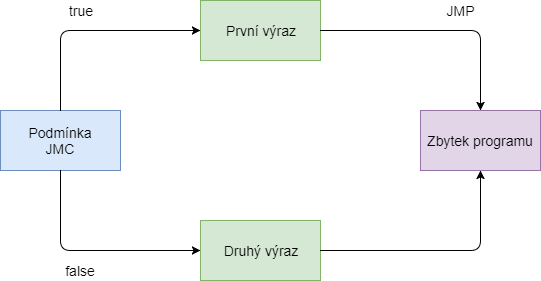
\includegraphics[width=\textwidth]{statementTernary.png}
\end{figure}

\paragraph{Příkaz if} -- pracuje se třídou Statementif, která obsahuje:
\begin{itemize}
\item \textbf{condition} -- podmínka
\item \textbf{statement} -- příkaz if
\item \textbf{elseStatement} příkaz else
\end{itemize}

Příkaz if vyhodnocuje podmínku, při pravdě vykoná příkaz if, jinak přeskočí na příkaz else, pokud existuje, jinak do zbytku programu. Implementace spočívá ve skoku JMC, kterým buď vykonáme příkaz if nebo skočíme do příkazu else. Pak jen stačí zajistit přidání skoku na konec if příkazu pro přeskočení else příkazu.

Příkaz if je ukázán na obrázku \ref{if}.

\begin{figure}[H]
\caption{Příkaz if}
\label{if}
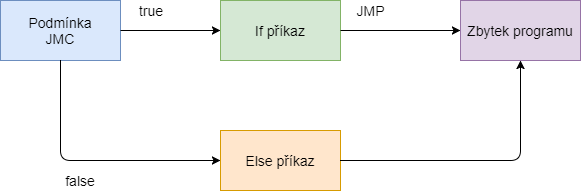
\includegraphics[width=\textwidth]{if.png}
\end{figure}

\paragraph{Příkaz while-do} -- pracuje s třídou StatementWhileDo, která obsahuje:
\begin{itemize}
\item \textbf{condition} -- podmínka
\item \textbf{statement} -- příkaz cyklus
\end{itemize}

Tento cyklus testuje podmínku na začátku cyklu. Pokud tato podmínka je pravdivá, provede cyklus. Pokud není, provede skok mimo cyklus do zbytku programu. Toto kompilujeme pomocí instrukce JMC. Na konec cyklu nyní stačí přidat instrukci skoku JMP, kterou se dostaneme zpátky na začátek k testování podmínky.

Cyklus while-do je zobrazen na obrázku \ref{whileDo}. 

\begin{figure}[H]
\caption{Cyklus while-do}
\label{whileDo}
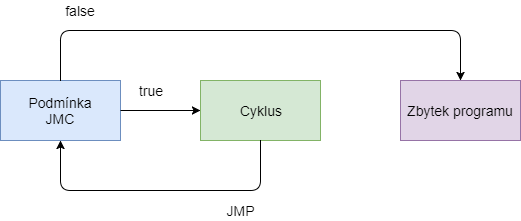
\includegraphics[width=\textwidth]{whileDo.png}
\end{figure}

\paragraph{Příkaz do-while} -- pracuje s třídou StatementDoWhile, která obsahuje:
\begin{itemize}
\item \textbf{condition} -- podmínka
\item \textbf{statement} -- příkaz cyklu
\end{itemize}

Tento cyklus testuje podmínku na konci cyklu. Nejdříve vykoná cyklus. Poté vyhodnotí podmínku. Pokud je pravdivá, potřebujeme skočit zpátky a pokud nepravdivá, tak pryč. Dosáhneme toho tak, že připravíme instrukci JMC a za ní instrukci skoku JMP. Skok JMP bude skákat vždy na začátek cyklu, tím dosáhneme toho, že při vyhodnocení podmínky pravdivě skočíme zpět. Nyní jen stačí nastavit JMC ven z cyklu, kam při nepravdě skočí do zbytku programu.

Cyklus do-while je zobrazen na obrázku \ref{doWhile}

\begin{figure}[H]
\caption{Cyklus do-while}
\label{doWhile}
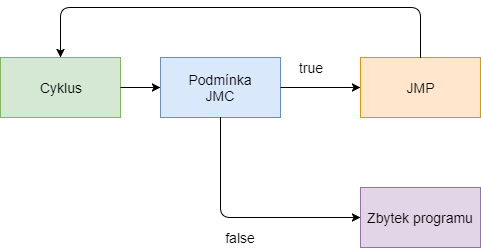
\includegraphics[width=\textwidth]{doWhile.png}
\end{figure}

\paragraph{Příkaz repeat-until} --  pracuje s třídou StatementRepeat, která obsahuje:
\begin{itemize}
\item \textbf{condition} -- podmínka
\item \textbf{statement} -- příkaz cyklu
\end{itemize}

Tento cyklus testuje podmínku na konci cyklu. Co ho odlišuje od cyklu do-while je to, že tento cyklus probíhá, dokud je podmínka nepravdivá. Toho dosáhneme jednoduše tak, že nám stačí skok JMC na začátek cyklu.

Cyklus repeat-until je zobrazen na obrázku \ref{repeatUntil}.

\begin{figure}[H]
\caption{Cyklus repeat-until}
\label{repeatUntil}
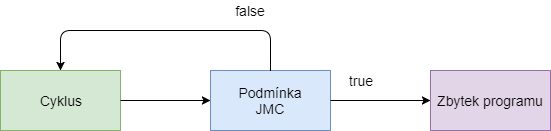
\includegraphics[width=\textwidth]{repeatUntil.png}
\end{figure}

\paragraph{Příkaz for} -- pracuje se třídou StatementFor, která obsahuje:
\begin{itemize}
\item \textbf{identifier} -- identifikátor iterační proměnné
\item \textbf{from} -- výraz dolní meze
\item \textbf{to} -- výraz horní meze
\item \textbf{statement} -- příkaz cyklus
\end{itemize}

For cyklus je nejsložitější cyklus v programu. Na rozdíl od ostatních zmíněných cyklů nekontroluje pouze podmínku, ale cyklus je řízen tzv. iterační proměnnou. Cyklus spočívá v následujících krocích:
\begin{enumerate}
\item Deklarace iterační proměnné, dolní a horní meze
\item Přiřazení dolní meze do iterační proměnné
\item Cyklus for vzrůstající:
\begin{enumerate}
\item Srovnání, jestli je iterační proměnná menší než horní mez
\item Pokud ano, proveďme cyklus, pokud ne, konec cyklu
\item Na konci cyklu připočtěme konstantní 1 k iterační proměnné
\item Skok zpět na srovnání
\end{enumerate}
\item Cyklus for klesající:
\begin{enumerate}
\item Srovnání, jestli je iterační proměnná větší než horní mez
\item Pokud ano, proveďme cyklus, pokud ne, konec cyklu
\item Na konci cyklu odečtěme konstatní 1 od iterační proměnné
\item Skok zpět na srovnání
\end{enumerate}
\end{enumerate}

Implementace cyklu postupuje podle tohoto návodu. Je deklarována iterační proměnná a získává hodnotu dolní meze. Tuto hodnotu je nutné uložit na zásobník, abychom jí mohli v průběhu cyklu měnit. V závislosti na typu for cyklu je je provedeno srovnání. Skokem JMC nyní budeme kontrolovat vykonání cyklu nebo výskok z cyklu pryč. Na konci cyklu již jen stačí přičíst/odečíst konstantní 1 a skokem JMP se vrátit do bodu srovnání.

Cyklus for je zobrazen na obrázku \ref{for}.

\begin{figure}[H]
\caption{Cyklus for}
\label{for}
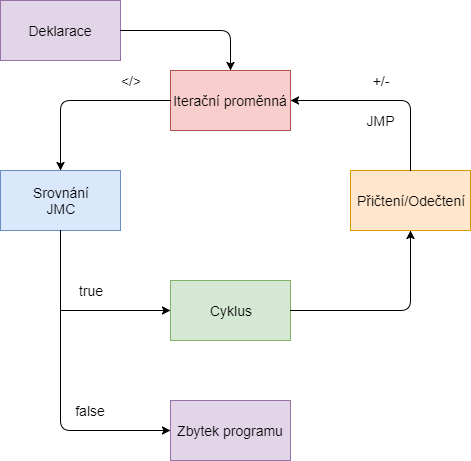
\includegraphics[width=\textwidth]{for.png}
\end{figure}

\paragraph{Příkaz case} -- pracuje se třídou StatementCase, která obsahuje:
\begin{itemize}
\item \textbf{expression} -- kontrolní výraz
\item \textbf{defaultStateemt} -- příkaz defaultní větve
\item \textbf{limbList} -- seznam objektů CaseLimb, jež obsahují:
\begin{itemize}
\item \textbf{statement} -- příkaz větve
\item \textbf{atomList} -- seznam objektů Atom
\end{itemize}
\end{itemize}

Příkaz case je nejsložitější příkaz v programu. Jde o obdobu příkazu if-else s tím rozdílem, že umožňuje definovat více větví s více možnostmi. Základní algoritmus pro příkaz case pascalovského typu byx mohl vypadat následovně:
\begin{enumerate}
\item Vyhodnoťme kontrolní výraz
\item Vezměme atomické hodnoty první větve. Srovnejme postupně s každou hodnotou kontrolní výraz, jestli se rovnají.
\item Pokud pro jednu z atomických hodnot vyhodnotíme pravdivě, vykonejme příkaz této větve, po tomto příkazu konec case. 
\item Pokud se ani jedna atomická hodnota nerovná s kontrolním výrazem, opakujeme pro další větve.
\item Pokud se výraz nerovná s žádnou atomickou hodnotou z žádných větví a neexistuje defaultní větev, program nic nevykoná, jinak vykoná defaultní větev.
\end{enumerate}

Při implementaci case postupujeme podle pravidel pascalovského case, které zde ještě zdůrazníme:
\begin{itemize}
\item Kontrolní výraz může být pouze číselného typu
\item Jedna větev může mít více atomických hodnot
\item Atomické hodnoty musejí být číselné
\item Po vykonání příkazu ve větvi program pokračuje za case příkazem
\item Podpora defaultní větve
\end{itemize}

Na začátku vyhodnotíme kontrolní výraz a uložíme ho na zásobník. Nyní budeme postupně procházet všechny větve a srovnávat výsledek kontrolního výrazu s atomickými hodnotami. 

Podívejme se na jednotlivá porovnávání. Zjistíme, jestli se kontrolní výraz rovná atomické hodnotě. Pokud se mu rovná, chceme přeskočit další vyhodnocování ostatních atomických výrazů ve stejné větvi a skočit rovnou do příkazové části. Jenže nemáme k dispozici instrukci skoku při hodnotě 1, tedy true, takže si vypomůžeme menším trikem - výsledek operace znegujeme a doplníme instrukci JMC. Nyní budeme skákat na příkazovou část větve při false, tedy srovnání bylo vyhodnoceno pravdivě, a při true, tedy srovnání bylo vyhodnoceno nepravdivě, pokračujeme na další atomickou hodnotu. 

Poslední atomická hodnota ve větvi je výjimkou od ostatních v tom, že při jejím vyhodnocení true, respektive false, potřebujeme skočit na další větev a tím se vyhnout příkazové části větve. Proto sem doplníme instrukci JMP. Tu samou instrukci doplníme i na konec příkazové části, abychom přeskočili zbylé větve a vyskočili z case příkazu (jde vlastně o automatickou obdobu break příkazu v jiných jazycích).

Po zkompilování všech větví se podíváme, jestli existuje defaultní větev. Pokud ano, zkompilujeme jí. Žádné atomické srovnání a skoky se zde neřeší. Po tomto je case příkaz hotov.

Příkaz case je ukázán na obrázku \ref{case}.

\begin{figure}[H]
\caption{Příkaz case}
\label{case}
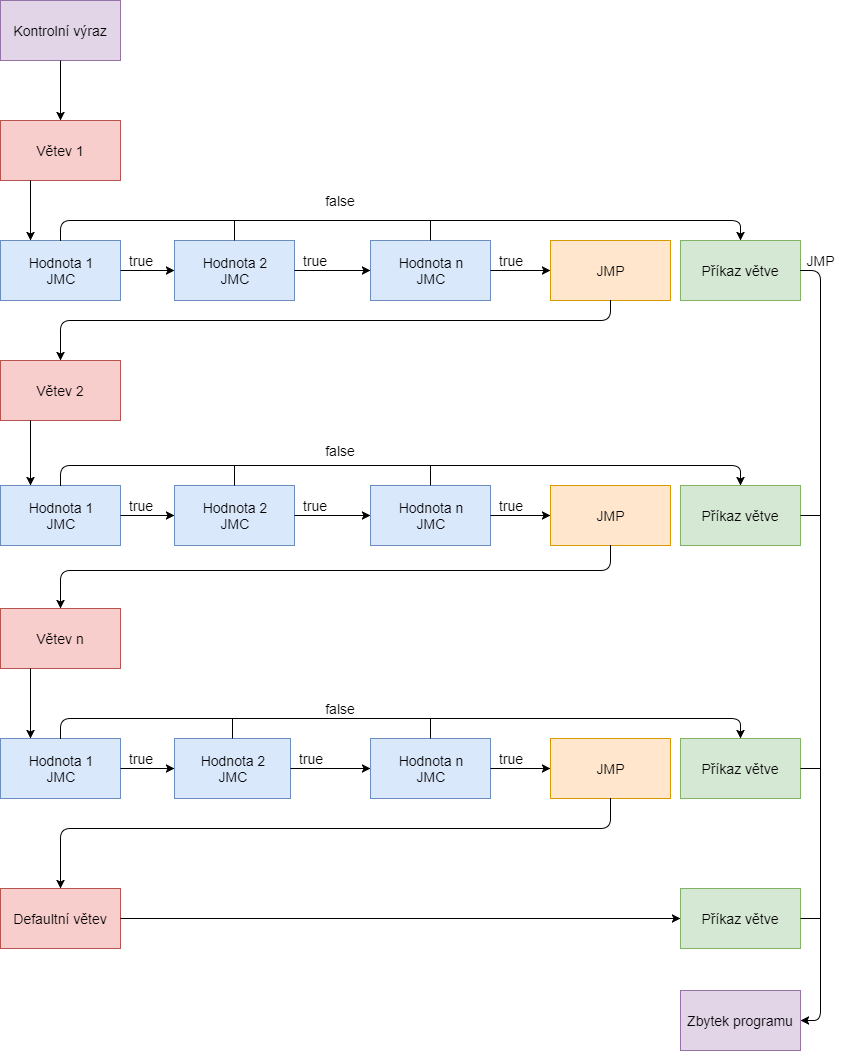
\includegraphics[width=\textwidth]{case.png}
\end{figure}

 
\section{Interpret}
Posledním krokem implementační části je vytvoření interpretu. Ten má za úkol správně interpretovat instrukce, které vytvoří překladač. Tyto instrukce jsou inspirovány instrukční sadou rozšířené PL/0. 

\subsection{Interpretace}
V balíku \texttt{interpret} se nachází 2 třídy, které slouží k interpretací:
\begin{itemize}
\item \textbf{Interpreter} -- představuje instanci interpretu 
\item \textbf{Stack} -- představuje zásobník a příslušné metody 
\end{itemize}

Interpretace funguje tak, že se postupným průchodem souboru provádějí jednotlivé instrukce, které jsou v souboru obsaženy. V podstatě se jedná o jeden velký přepínač--switch, ve kterém se podle názvu instrukce provede to, co má. Většina základních instrukcí se shoduje s těmi, kterými disponuje základní i rozšířená verze jazyka PL/0. Protože jsme se rozhodli pro implementaci reálných čísel v \texttt{IEEE-format} bylo nutné pro tyto čísla vytvořit nové instrukce. Díky tomu je možné reálné číslo uložit pouze na jednu pozici v zásobníku.
\begin{itemize}
\item LRT -- vloží konstantní reálnou hodnotu 
\item LOR -- načte reálnou hodnotu vrcholu
\item STR -- uloží reálnou hodnotu vrcholu
\item RER -- načte reálné číslo ze vstupu a uloží jej na zásobník
\item WRR -- odebere reálné číslo z vrcholu zásobníku a vypíše jej na vstup
\end{itemize}
\subsection{Instrukční sada}
Pro úplnost, v tabulce \ref{instrukce} jsou uvedeny všechny instrukce a jejich popis, co interpret podporuje.
\begin{longtable}{|c|l|p{10cm}|}
\caption{Instrukce}
\label{instrukce}
\endfirsthead
\endhead
\hline
		Kód & Instrukce & Popis \\
\hline\hline
\rule{0pt}{3ex}1 & \texttt{LIT 0, M} & Vloží konstantní celou hodnotu (\texttt{literál}) \texttt{M} do zásobníku \\ \hline
\rule{0pt}{3ex}2 & \texttt{LRT 0, M} & Vloží konstantní reálnou hodnotu (\texttt{literál}) \texttt{M} do zásobníku \\ \hline
\rule{0pt}{3ex}3 & \texttt{OPR 0, M} & \textbf{Operace}, která se provede nad vrcholem zásobníku \textbf{pro celé čísla} \\ \hline
\rule{0pt}{3ex} & \texttt{OPR 0, 1} & \textbf{Negace}; vybere vrchol a vrátí negativní hodnotu \\ \hline
\rule{0pt}{3ex} & \texttt{OPR 0, 2} & \textbf{Sčítání}; vybere dvě hodnoty, sečte a vrátí \\ \hline
\rule{0pt}{3ex} & \texttt{OPR 0, 3} & \textbf{Odečítání}; vybere dvě hodnoty, odečte druhou první a vrátí výsledek \\ \hline
\rule{0pt}{3ex} & \texttt{OPR 0, 4} & \textbf{Násobení}; vybere dvě hodnoty, vynásobí a vrátí výsledek \\ \hline
\rule{0pt}{3ex} & \texttt{OPR 0, 5} & \textbf{Dělení}; vybere dvě hodnoty, vydělí druhou první \\ \hline
\rule{0pt}{3ex} & \texttt{OPR 0, 6} & \textbf{Lichost}; vybere vrchol a vloží 1 když liché, 0 když sudé \\ \hline
\rule{0pt}{3ex} & \texttt{OPR 0, 7} & \textbf{Modulo}; vybere dvě hodnoty, vydělí druhý prvním a vloží zbytek \\ \hline
\rule{0pt}{3ex} & \texttt{OPR 0, 8} & \textbf{Rovnost}; vybere dvě hodnoty, a vloží 1 pokud se rovnají, jinak 0 \\ \hline
\rule{0pt}{3ex} & \texttt{OPR 0, 9} & \textbf{Nerovnost}; vybere dvě hodnoty a vloží 0 pokud se rovnají, jinak 0 \\ \hline
\rule{0pt}{3ex} & \texttt{OPR 0, 10} & \textbf{Menší než}; vybere dvě hodnoty a vloží 1 pokud je první menší než druhá, jinak 0 \\ \hline
\rule{0pt}{3ex} & \texttt{OPR 0, 11} & \textbf{Větší nebo rovno než}; vybere dvě hodnoty a vloží 1 pokud je první větší nebo rovno než druhá, jinak 0 \\ \hline
\rule{0pt}{3ex} & \texttt{OPR 0, 12} & \textbf{Větší}; vybere dvě hodnoty a vloží 1 pokud je první větší nebo rovno než druhá, jinak 0 \\ \hline
\rule{0pt}{3ex} & \texttt{OPR 0, 13} & \textbf{Menší nebo rovno než}; vybere dvě hodnoty a vloží 1 pokud je první menší nebo rovno než druhá, jinak 0 \\ \hline
\rule{0pt}{3ex}4 & \texttt{LOD L, M} & \textbf{Načtení}; načte hodnotu vrcholu z umístění dané offsetem M od L lexikografických úrovní dolů \\ \hline
\rule{0pt}{3ex}5 & \texttt{STO L, M} & \textbf{Uložení}; uloží hodnotu vrcholu z umístění dané offsetem M od L lexikografických úrovní dolů \\ \hline
\rule{0pt}{3ex}4 & \texttt{LOR L, M} & \textbf{Načtení}; načte reálnou hodnotu vrcholu z umístění dané offsetem M od L lexikografických úrovní dolů \\ \hline
\rule{0pt}{3ex}5 & \texttt{STR L, M} & \textbf{Uložení}; uloží reálnou hodnotu vrcholu z umístění dané offsetem M od L lexikografických úrovní dolů \\ \hline
\rule{0pt}{3ex}6 & \texttt{CAL L, M} & \textbf{Volání procedury} v kódovém indexu \textbf{M} \\ \hline
\rule{0pt}{3ex}7 & \texttt{RET 0, 0} & \textbf{Návrat z procedury}; vrátí se z procedury do volající procedury \\ \hline
\rule{0pt}{3ex}8 & \texttt{INT 0, M} & \textbf{Alokování} místa pro M hodnot na vrcholo zásobníku \\ \hline
\rule{0pt}{3ex}9 & \texttt{JMP 0, M} & Provede skok do instrukce \textbf{M} \\ \hline
\rule{0pt}{3ex}10 & \texttt{JMC 0, M} & Vybere vrchol a skočí k instrukci M pokud je rovna 0, \textbf{podmíněný skok} \\ \hline
\rule{0pt}{3ex}11 & \texttt{REA L, M} & \textbf{Načte celé číslo} ze vstupu a uloží jej na zásobník \\ \hline
\rule{0pt}{3ex}12 & \texttt{WRI L, M} & Odebere celé číslo z vrcholu zásobníku a \textbf{vypíše jej na vstup} \\ \hline
\rule{0pt}{3ex}13 & \texttt{RER L, M} & \textbf{Načte reálné číslo} ze vstupu a uloží jej na zásobník \\ \hline
\rule{0pt}{3ex}14 & \texttt{WRR L, M} & Odebere reálné číslo z vrcholu zásobníku a \textbf{vypíše jej na vstup} \\ \hline
\rule{0pt}{3ex}15 & \texttt{OPF 0, M} & \textbf{Operace}, která se provede nad vrcholem zásobníku \textbf{pro reálná čísla} \\ \hline
\rule{0pt}{3ex} & \texttt{OPF 0, 1} & \textbf{Negace}; vybere vrchol a vrátí negativní hodnotu \\ \hline
\rule{0pt}{3ex} & \texttt{OPF 0, 2} & \textbf{Sčítání}; vybere dvě hodnoty, sečte a vrátí \\ \hline
\rule{0pt}{3ex} & \texttt{OPF 0, 3} & \textbf{Odečítání}; vybere dvě hodnoty, odečte druhou první a vrátí výsledek \\ \hline
\rule{0pt}{3ex} & \texttt{OPF 0, 4} & \textbf{Násobení}; vybere dvě hodnoty, vynásobí a vrátí výsledek \\ \hline
\rule{0pt}{3ex} & \texttt{OPF 0, 5} & \textbf{Dělení}; vybere dvě hodnoty, vydělí druhou první \\ \hline
\rule{0pt}{3ex} & \texttt{OPF 0, 6} & \textbf{Lichost}; vybere vrchol a vloží 1 když liché, 0 když sudé \\ \hline
\rule{0pt}{3ex} & \texttt{OPF 0, 7} & \textbf{Modulo}; vybere dvě hodnoty, vydělí druhý prvním a vloží zbytek \\ \hline
\rule{0pt}{3ex} & \texttt{OPF 0, 8} & \textbf{Rovnost}; vybere dvě hodnoty, a vloží 1 pokud se rovnají, jinak 0 \\ \hline
\rule{0pt}{3ex} & \texttt{OPF 0, 9} & \textbf{Nerovnost}; vybere dvě hodnoty a vloží 0 pokud se rovnají, jinak 0 \\ \hline
\rule{0pt}{3ex} & \texttt{OPF 0, 10} & \textbf{Menší než}; vybere dvě hodnoty a vloží 1 pokud je první menší než druhá, jinak 0 \\ \hline
\rule{0pt}{3ex} & \texttt{OPF 0, 11} & \textbf{Větší nebo rovno než}; vybere dvě hodnoty a vloží 1 pokud je první větší nebo rovno než druhá, jinak 0 \\ \hline
\rule{0pt}{3ex} & \texttt{OPF 0, 12} & \textbf{Větší}; vybere dvě hodnoty a vloží 1 pokud je první větší nebo rovno než druhá, jinak 0 \\ \hline
\rule{0pt}{3ex} & \texttt{OPF 0, 13} & \textbf{Menší nebo rovno než}; vybere dvě hodnoty a vloží 1 pokud je první menší nebo rovno než druhá, jinak 0 \\ \hline
\rule{0pt}{3ex} 16 & \texttt{RTI 0, 0} & \textbf{Reálné číslo na celé číslo}; vybere jednu hodnotu ze zásobníku a vloží celou část čísla do zásobníku \\ \hline
\rule{0pt}{3ex} 17 & \texttt{ITR 0, 0} & \textbf{Celé číslo na reálné číslo}; vybere jednu hodnotu ze zásobníku a vloží číslo jako reálné do zásobníku \\ \hline
\rule{0pt}{3ex} 18 & \texttt{NEW 0, 0} &  \textbf{Alokace na haldě}; alokuje se jedno místo na haldě, na zásobník vloží hodnotu představující pozici místa v haldě \\ \hline
\rule{0pt}{3ex} 19 & \texttt{DEL 0, 0} & \textbf{Uvolnění místa na haldě}; odebere ze zásobníku jednu hodnotu a to adresu na haldě, kterou uvolní \\ \hline
\rule{0pt}{3ex} 20 & \texttt{LDA 0, 0} & \textbf{Načtení hodnoty z haldy}; odebere ze zásobníku hodnotu a vloží hodnotu z haldy \\ \hline
\rule{0pt}{3ex} 21 & \texttt{STA 0, 0} & \textbf{Uložení hodnoty na haldu}; odebere dvě hodnoty zásobníku. Na první představující adresu uloží druhou v haldě \\ \hline
\rule{0pt}{3ex} 22 & \texttt{PLD 0, 0} & \textbf{Dynamické načtení hodnoty z místa určeného L/A}; odebere ze zásobníku dvě hodnoty. První je úroveň zanoření a druhá je relativní pozice. Z té se načte hodnota na vrchol zásobníku  \\ \hline
\rule{0pt}{3ex} 23 & \texttt{PST 0, 0} & \textbf{Dynamické uložení hodnoty z místa určeného L/A}; odebere ze zásobníku tři hodnoty. První je úroveň zanoření, druhá relativní pozice a třetí odebraná hodnota představuje hodnotu k uložení \\ \hline
\end{longtable}
\section{Chyby programu}
Program při vykonávání může narazit na několik různých chyb při překladu. Problémy nalezené při analýze řeší ANTLR a program je pouze zachycuje a vyhazuje jako výjimku. Chyby při syntéze a interpretaci jsou již v rukách tvůrců a tak byly sestaveny jednotlivé chyby, jejich kód a popis chyby. Program zároveň vrací tento kód chyby jako svůj návratový kód. Tyto chyby jsou zaneseny do tabulky \ref{chyby}.

\begin{longtable}{|c|p{5.5cm}|p{6.5cm}|}
\caption{Chybové kódy}
\label{chyby}
\endfirsthead
\endhead
\hline
		\textbf{Kód} & \textbf{Chyba} & \textbf{Komentář} \\
\hline\hline
\rule{0pt}{3ex}0 & \texttt{Žádná chyba} & Program proběhl správně \\ \hline
\multicolumn{3}{|l|}{\textbf{Překladač}}\\ \hline
\rule{0pt}{3ex}1 & \texttt{Variable not initialized} & Použili jste hodnotu předtím, než byla inicializována \\ \hline
\rule{0pt}{3ex}2 & \texttt{Variable already declared} & Pokoušíte se deklarovat proměnnou, která již byla deklarována \\ \hline
\rule{0pt}{3ex}3 & \texttt{Constant reassign} & Pokoušíte se změnit hodnotu konstanty \\ \hline
\rule{0pt}{3ex}4 & \texttt{Unknown identifier} & Vyskytl se neznámý identifikátor \\ \hline
\rule{0pt}{3ex}5 & \texttt{Unknown label} & Vyskytlo se neznámé návěští \\ \hline
\rule{0pt}{3ex}6 & \texttt{Unknown procedure} & Vyskytla se neznámá procedura \\ \hline
\rule{0pt}{3ex}7 & \texttt{Parallel declaration number mismatch} & Paralelní deklarace vyžaduje stejný počet proměnných a výrazů\\ \hline
\rule{0pt}{3ex}8 & \texttt{Incompatible types} & Typový výsledek výrazu neodpovídá očekávanému typu \\ \hline
\rule{0pt}{3ex}9 & \texttt{Expression variable type mismatch} & Ve výrazu se vyskytly neslučitelné typy \\ \hline
\rule{0pt}{3ex}10 & \texttt{Strict mode expression variable type mismatch} & Striktní mód nedovoluje smíšení různých typů ve výrazu \\ \hline
\rule{0pt}{3ex}11 & \texttt{Can not assign loop variable} & Nepoužil jste unikátní proměnnou jako iterační proměnnou \texttt{for} cyklu \\ \hline
\rule{0pt}{3ex}12 & \texttt{Label used elsewhere} & Návěští již bylo použito jinde \\ \hline
\rule{0pt}{3ex}13 & \texttt{Label out of reach} & Návěští je mimo dosah \\ \hline
\rule{0pt}{3ex}14 & \texttt{Label never used} & Skáčete na návěští, které není v programu použito \\ \hline
\rule{0pt}{3ex}15 & \texttt{Label not allowed in for cycle} & Návěští není povoleno ve \texttt{for} cyklu \\ \hline
\rule{0pt}{3ex}16 & \texttt{No boolean type in case} & \texttt{Case} větev nepodporuje logický datový typ \\ \hline
\rule{0pt}{3ex}17 & \texttt{Case atom used multiple times} & Definujete \texttt{case} větev, která již byl použita \\ \hline
\rule{0pt}{3ex}18 & \texttt{Legacy mode only allows var type} & \texttt{Legacy} mód povoluje pouze typ \texttt{var} \\ \hline
\rule{0pt}{3ex}19 & \texttt{Legacy mode real constant not allowed} & \texttt{Legacy} mód nepovoluje konstatní reálné číslo \\ \hline
\rule{0pt}{3ex}20 & \texttt{Legacy mode boolean constant not allowed} & \texttt{Legacy} mód nepovoluje logickou konstantu \\ \hline
\rule{0pt}{3ex}21 & \texttt{Legacy mode logical expression not allowed} & \texttt{Legacy} mód nepovoluje logické výrazy \\ \hline
\rule{0pt}{3ex}22 & \texttt{Legacy mode negation expression not allowed} & \texttt{Legacy} mód nepovoluje výraz negace \\ \hline
\rule{0pt}{3ex}23 & \texttt{Non legacy mode var type not allowed} & \texttt{Var} typ není povolen v \texttt{non-legacy} módu \\ \hline
\multicolumn{3}{|l|}{\textbf{Interpret}}\\ \hline
\rule{0pt}{3ex}24 & \texttt{Stack overflow} & Došlo k přetečení zásobníku \\ \hline
\rule{0pt}{3ex}25 & \texttt{Stack underflow} & Došlo k podtečení zásobníku \\ \hline
\rule{0pt}{3ex}26 & \texttt{Unknown instruction} & Tato instrukce není známa \\ \hline
\rule{0pt}{3ex}27 & \texttt{Program counter is out of range} & Čítač instrukcí je mimo rozsah \\ \hline
\end{longtable}

\chapter{Testování}

Program byl kromě pečlivého ručního otestování autorů otestován sadou automatických funkcionálních testů za podpory knihovny JUnit. Veškeré třídy se nacházejí v balíku \textit{test.zcu.cz.kiv.fjp} a veškeré testovací soubory ve složce \textit{testFiles}.

\section{ANTLR}
Testování ANTLR, potažmo analytické části překladače, je o otestování, že přijmeme správné vstupy a odmítneme nesprávné. Jde tedy o testování funkčnosti pravidel gramatiky. Správně vstupy jsou předpokladem pro další část překladu a proto byla věnována zvýšená pozornost této části testování. 

Jednotlivé testovací třídy jsou v balíku \textit{ANTLR}.
\begin{itemize}
\item \textbf{TestProgram} - testovací sada na základní vlastnosti programu týkající se především hlavičky programu.
\item \textbf{TestDeclarations} - testovací sada na deklarace. Důraz kladen na správné přijetí všech druhů deklarací včetně všech jejich povolených tvarů.
\item \textbf{TestExpressions} - testování vlastností výrazů. Kontrola, že dodržují předepsaná pravidla o počtu výrazů, povolené symboly, klíčová slova apod.
\item \textbf{TestStatements} - testovací sada na příkazy. Správné tvary všech příkazů včetně návěští.
\item \textbf{TestSuiteANTLR} - testovací sada, která spustí všechny zmíněné testy.
\end{itemize} 

\section{Překladač}

Testování samotného překladače je složitý problém. Nasnadě je využít přeložené instrukce pro další budoucí testování. Jenže to vyvolává mnohem více otázek než zodpovídá. Kde tyto instrukce vezmeme? Náš překladač podporuje velké množství příkazů, mnohem více než PL/0, navíc využívá vlastní instrukce pro převod čísel a reprezentaci reálného čísla. Musel by se tedy použít samotný překladač. To by znamenalo srovnávat starší výsledek překladače s novými výsledky překladače. Smysl takového testování je velice malý. Přes srovnávání instrukcí otestování překladače nevede. 


Zaměřme se nejdříve na to, co testovat snadno lze - otestování chybových stavů. Překladač při naražení na problém, vyvolá chybový stav, vypíše chybovou hlášku na konzoli a ukončí program přes \textit{System.exit}. Návratová hodnota tohoto volání odpovídá číslu chyby uvedené v tabulce \ref{chyby}. Knihovna JUnit neumožňuje testovat tuto návratovou hodnotu a tak si vypomůžeme další knihovnou, která tuto funkcionalitu do JUnit doplńuje - \textit{System rules}. 

V balíku \textit{compiler} se nachází \textbf{TestErrors}. Tato třída průběžne otestuje správnou reakci překladače na chybné vstupy kontrolou návratové hodnoty \textit{System.exit} pomocí výše popsané knihovny.

Další třídou je \textbf{TestComplex}. Tato třída testuje komplexnější programy. Bez výpomoci třetího si zde nepomůžeme a tak toto testování probíhá za asistence interpretu. Všechny testy využívají předpřipravená data ve třídě \textbf{TestData}. Všechny programy vždy vypisují výsledek pomocí instrukcí pro I/O, a právě tyto výstupy poté kontrolujeme v testovacích sadách. 

V rozhodovacích problémech odpovídají programy buď \textbf{1} (ano) nebo \textbf{-1} (ne).

Testujeme následující programy:

\begin{itemize}
\item \textbf{armstrong} - Program rozhodune o zadaném čísle, jestli se jedná o Armstrongovo číslo.
\item \textbf{factorial} - Program vypočítává faktoriál zadaného čísla.
\item \textbf{fahrenheit} - Program převádí zadané číslo z celsia do fahrenheit.
\item \textbf{fibonacci} - Program vypíše prvních \textit{n} čísel Fibonacciho posloupnosti.
\item \textbf{palindrome} - Program rozhodne o zadaném čísle, jestli se jedná o palindrom.
\item \textbf{prime} - Program rozhodne o zadaném čísle, jestli se jedná o prvočíslo.
\end{itemize}

Všechny testovací sady překladače lze spustit najednou pomocí třídy \textbf{TestSuiteCompiler}.

\section{Interpret}

\chapter{Uživatelská dokumentace} 

\section{Postup přeložení a sestavení}

\section{Používání programu}

\chapter{Závěr}

\section{Nedosažené cíle}
Od původní analýzy se implementovaný program liší ve dvou věcech.

 Za prvé původním cílem byl překlad našeho jazyka do instrukcí PL/0. To bylo splněno částečně vzhledem k tomu, že pro realizaci překladu reálných čísel byly použity vlastní instrukce a nikoli instrukce rozšířené PL/0.
 
 Za druhé nebyl realizován datový typ řetězec. Z důvodů časové tísně a dalších povinností byla implementace tohoto datového typu nejdříve odložena načež zrušena. 

\section{Omezení}

I přes implementaci některý funkcí jsou tyto funkce omezené v určitých aspektech:

\begin{itemize}
\item Návěští musí být použito pouze na začátku příkazu. To sebou nese určitá omezení v případě nutnosti skočit z cyklu ven, pokud za tímto cyklem nic není.
\item Hlavička \textit{program(název)} je vyžadována i přesto, že v programu ničemu neslouží.
\item I/O příkazy nepodporují konstanty
\item Překladač nepodporuje logické konstanty v číselných výrazech (pouze v logických)
\item Iterační proměnná \textit{for} cyklu musí být nedeklarována
\item \textit{Case} pracuje pouze s číselnými typy
\item Konstanta může být pouze atomická
\item Deklarovat proměnné lze pouze v deklarační části
\end{itemize}

\section{Dosažené cíle}

Hlavní předsevzatý cíl bylo splnit zadání, tedy vytvořit překladač vlastního jazyka. Tento cíl byl později doplněn o vlastní interpret. Překladač i interpret byly otestovány automatickými testy na jednoduchých i složitějších případech. Funkcionalitu programu shrňme v následujícím seznamu:
\begin{itemize}
\item Programový mód - \textit{legacy}, \textit{default}, \textit{strict}
\item \textbf{Deklarace}
\begin{itemize}
\item Deklarace konstant
\item Deklarace návěští
\item Deklarace proměnných
\item Deklarace paralelních proměnných
\item Deklarace procedury
\end{itemize}
\item \textbf{Výrazy}
\begin{itemize}
\item Unární mínus
\item Lichost
\item Negace
\item Násobení, dělení, modulo
\item Sčítání, odčítání
\item Srovnání
\end{itemize}
\item \textbf{Příkazy}
\begin{itemize}
\item I/O příkaz
\item Příkaz přiřazení
\item Ternární příkaz
\item Goto příkaz
\item Volání procedury
\item Blokový příkaz (\textit{begin end})
\item Cyklus \textit{do while}
\item Cyklus \textit{while do}
\item Cyklus \textit{repeat until}
\item Cyklus \textit{for}
\item Příkaz podmínky \textit{if}
\item Příkaz větvení \textit{case}
\end{itemize}
\item \textbf{Interpret podporuje}
\begin{itemize}
\item Základní PL/0
\item Rozšířená PL/0
\item Naše instrukce pro reálná čísla
\end{itemize}
\end{itemize}


\end{document}